% Options for packages loaded elsewhere
\PassOptionsToPackage{unicode}{hyperref}
\PassOptionsToPackage{hyphens}{url}
%
\documentclass[
]{book}
\usepackage{lmodern}
\usepackage{amssymb,amsmath}
\usepackage{ifxetex,ifluatex}
\ifnum 0\ifxetex 1\fi\ifluatex 1\fi=0 % if pdftex
  \usepackage[T1]{fontenc}
  \usepackage[utf8]{inputenc}
  \usepackage{textcomp} % provide euro and other symbols
\else % if luatex or xetex
  \usepackage{unicode-math}
  \defaultfontfeatures{Scale=MatchLowercase}
  \defaultfontfeatures[\rmfamily]{Ligatures=TeX,Scale=1}
\fi
% Use upquote if available, for straight quotes in verbatim environments
\IfFileExists{upquote.sty}{\usepackage{upquote}}{}
\IfFileExists{microtype.sty}{% use microtype if available
  \usepackage[]{microtype}
  \UseMicrotypeSet[protrusion]{basicmath} % disable protrusion for tt fonts
}{}
\makeatletter
\@ifundefined{KOMAClassName}{% if non-KOMA class
  \IfFileExists{parskip.sty}{%
    \usepackage{parskip}
  }{% else
    \setlength{\parindent}{0pt}
    \setlength{\parskip}{6pt plus 2pt minus 1pt}}
}{% if KOMA class
  \KOMAoptions{parskip=half}}
\makeatother
\usepackage{xcolor}
\IfFileExists{xurl.sty}{\usepackage{xurl}}{} % add URL line breaks if available
\IfFileExists{bookmark.sty}{\usepackage{bookmark}}{\usepackage{hyperref}}
\hypersetup{
  pdftitle={Fundamentals of Spatial Analysis in R},
  pdfauthor={Marc Weber},
  hidelinks,
  pdfcreator={LaTeX via pandoc}}
\urlstyle{same} % disable monospaced font for URLs
\usepackage{color}
\usepackage{fancyvrb}
\newcommand{\VerbBar}{|}
\newcommand{\VERB}{\Verb[commandchars=\\\{\}]}
\DefineVerbatimEnvironment{Highlighting}{Verbatim}{commandchars=\\\{\}}
% Add ',fontsize=\small' for more characters per line
\usepackage{framed}
\definecolor{shadecolor}{RGB}{248,248,248}
\newenvironment{Shaded}{\begin{snugshade}}{\end{snugshade}}
\newcommand{\AlertTok}[1]{\textcolor[rgb]{0.94,0.16,0.16}{#1}}
\newcommand{\AnnotationTok}[1]{\textcolor[rgb]{0.56,0.35,0.01}{\textbf{\textit{#1}}}}
\newcommand{\AttributeTok}[1]{\textcolor[rgb]{0.77,0.63,0.00}{#1}}
\newcommand{\BaseNTok}[1]{\textcolor[rgb]{0.00,0.00,0.81}{#1}}
\newcommand{\BuiltInTok}[1]{#1}
\newcommand{\CharTok}[1]{\textcolor[rgb]{0.31,0.60,0.02}{#1}}
\newcommand{\CommentTok}[1]{\textcolor[rgb]{0.56,0.35,0.01}{\textit{#1}}}
\newcommand{\CommentVarTok}[1]{\textcolor[rgb]{0.56,0.35,0.01}{\textbf{\textit{#1}}}}
\newcommand{\ConstantTok}[1]{\textcolor[rgb]{0.00,0.00,0.00}{#1}}
\newcommand{\ControlFlowTok}[1]{\textcolor[rgb]{0.13,0.29,0.53}{\textbf{#1}}}
\newcommand{\DataTypeTok}[1]{\textcolor[rgb]{0.13,0.29,0.53}{#1}}
\newcommand{\DecValTok}[1]{\textcolor[rgb]{0.00,0.00,0.81}{#1}}
\newcommand{\DocumentationTok}[1]{\textcolor[rgb]{0.56,0.35,0.01}{\textbf{\textit{#1}}}}
\newcommand{\ErrorTok}[1]{\textcolor[rgb]{0.64,0.00,0.00}{\textbf{#1}}}
\newcommand{\ExtensionTok}[1]{#1}
\newcommand{\FloatTok}[1]{\textcolor[rgb]{0.00,0.00,0.81}{#1}}
\newcommand{\FunctionTok}[1]{\textcolor[rgb]{0.00,0.00,0.00}{#1}}
\newcommand{\ImportTok}[1]{#1}
\newcommand{\InformationTok}[1]{\textcolor[rgb]{0.56,0.35,0.01}{\textbf{\textit{#1}}}}
\newcommand{\KeywordTok}[1]{\textcolor[rgb]{0.13,0.29,0.53}{\textbf{#1}}}
\newcommand{\NormalTok}[1]{#1}
\newcommand{\OperatorTok}[1]{\textcolor[rgb]{0.81,0.36,0.00}{\textbf{#1}}}
\newcommand{\OtherTok}[1]{\textcolor[rgb]{0.56,0.35,0.01}{#1}}
\newcommand{\PreprocessorTok}[1]{\textcolor[rgb]{0.56,0.35,0.01}{\textit{#1}}}
\newcommand{\RegionMarkerTok}[1]{#1}
\newcommand{\SpecialCharTok}[1]{\textcolor[rgb]{0.00,0.00,0.00}{#1}}
\newcommand{\SpecialStringTok}[1]{\textcolor[rgb]{0.31,0.60,0.02}{#1}}
\newcommand{\StringTok}[1]{\textcolor[rgb]{0.31,0.60,0.02}{#1}}
\newcommand{\VariableTok}[1]{\textcolor[rgb]{0.00,0.00,0.00}{#1}}
\newcommand{\VerbatimStringTok}[1]{\textcolor[rgb]{0.31,0.60,0.02}{#1}}
\newcommand{\WarningTok}[1]{\textcolor[rgb]{0.56,0.35,0.01}{\textbf{\textit{#1}}}}
\usepackage{longtable,booktabs}
% Correct order of tables after \paragraph or \subparagraph
\usepackage{etoolbox}
\makeatletter
\patchcmd\longtable{\par}{\if@noskipsec\mbox{}\fi\par}{}{}
\makeatother
% Allow footnotes in longtable head/foot
\IfFileExists{footnotehyper.sty}{\usepackage{footnotehyper}}{\usepackage{footnote}}
\makesavenoteenv{longtable}
\usepackage{graphicx,grffile}
\makeatletter
\def\maxwidth{\ifdim\Gin@nat@width>\linewidth\linewidth\else\Gin@nat@width\fi}
\def\maxheight{\ifdim\Gin@nat@height>\textheight\textheight\else\Gin@nat@height\fi}
\makeatother
% Scale images if necessary, so that they will not overflow the page
% margins by default, and it is still possible to overwrite the defaults
% using explicit options in \includegraphics[width, height, ...]{}
\setkeys{Gin}{width=\maxwidth,height=\maxheight,keepaspectratio}
% Set default figure placement to htbp
\makeatletter
\def\fps@figure{htbp}
\makeatother
\setlength{\emergencystretch}{3em} % prevent overfull lines
\providecommand{\tightlist}{%
  \setlength{\itemsep}{0pt}\setlength{\parskip}{0pt}}
\setcounter{secnumdepth}{5}
\usepackage{booktabs}
\usepackage[]{natbib}
\bibliographystyle{plainnat}

\title{Fundamentals of Spatial Analysis in R}
\author{Marc Weber}
\date{2020-08-04}

\begin{document}
\maketitle

{
\setcounter{tocdepth}{1}
\tableofcontents
}
\hypertarget{intro}{%
\chapter{Introduction}\label{intro}}

\begin{figure}
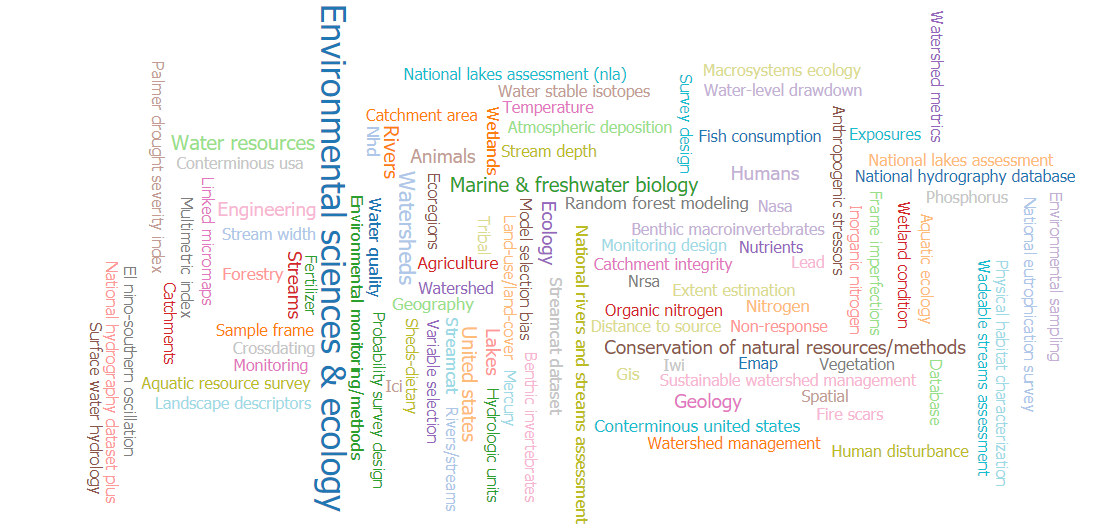
\includegraphics[width=1\linewidth]{images/WordCloud} \caption{A bit about me}\label{fig:unnamed-chunk-1}
\end{figure}

\begin{itemize}
\item
  Workshop agenda

  \begin{itemize}
  \tightlist
  \item
    Intro and quick review of basic R objects and methods
  \item
    Getting spatial data into R
  \item
    Learning ways to map and visualize spatial data
  \item
    Understanding coordinate reference systems (CRS)!
  \item
    Along the way: overview of select \texttt{tidyverse} packages and syntax

    \begin{itemize}
    \tightlist
    \item
      i.e.~\texttt{ggplot2}, \texttt{dplyr}, \texttt{readr}, \texttt{tidyr}, the pipe operator \%\textgreater\%
    \end{itemize}
  \item
    Working with vector and raster data in R
  \item
    If this is all new, don't sweat it - google things, we'll answer questions as we go
  \end{itemize}
\item
  This portion of workshop there is no expectation of experience with spatial analysis in R - if you already have some experience, you are sure to pick up new tricks - if you don't, we'll cover the basics
\item
  We have a limited time to cover a very broad topic, so I'll move quickly - ask questions as they come up, but if you get lost on steps we'll have time for discussion at the end and material will be available to peruse at your own speed later.
\end{itemize}

\hypertarget{workshop-packages-and-data}{%
\section{Workshop Packages and Data}\label{workshop-packages-and-data}}

\begin{itemize}
\item
  Packages you need installed

  \begin{itemize}
  \tightlist
  \item
    \texttt{sf}
  \item
    \texttt{raster}
  \item
    \texttt{stars}
  \item
    \texttt{tmap}
  \item
    \texttt{tmaptools}
  \item
    \texttt{dplyr}
  \item
    \texttt{devtools}
  \item
    \texttt{palmerpenguins}
  \item
    \texttt{tigris}
  \item
    \texttt{tibble}
  \item
    \href{https://github.com/mhweber/awra2020spatial}{awra2020spatial} - data for this workshop contained in package
  \end{itemize}
\item
  Downloading content via Github
\item
  Using RMarkdown and RStudio
\end{itemize}

\hypertarget{overview}{%
\subsection{Overview}\label{overview}}

\begin{figure}
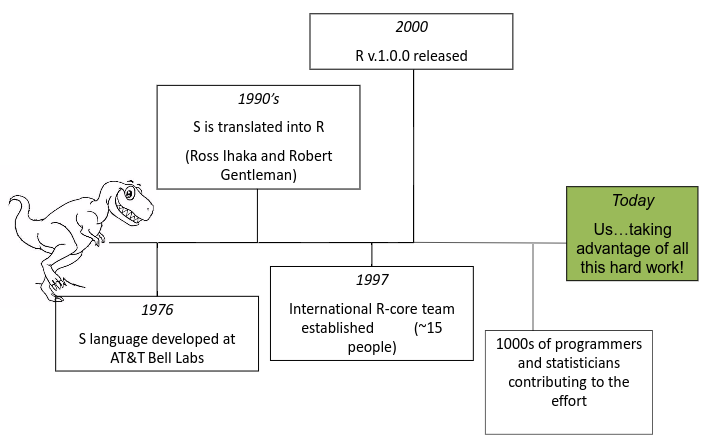
\includegraphics[width=1.5\linewidth]{images/History of R} \caption{History of R}\label{fig:unnamed-chunk-2}
\end{figure}

What is R and why should we use R for spatial analysis? Let's break that into two questions - first, what is R and why should we use it?

\begin{itemize}
\tightlist
\item
  A language and environment for statistical computing and graphics
\item
  R is lightweight, free, open-source and cross-platform
\item
  Works with contributed packages - currently 15,362 - extensibility
\item
  Automation and recording of workflow (reproducibility)
\item
  Optimized work flow - data manipulation, analysis and visualization all in one place
\item
  R does not alter underlying data - manipulation and visualization in memory
\item
  R is great for repetetive graphics
\end{itemize}

Second, why use R for spatial, or GIS, work?

\begin{itemize}
\tightlist
\item
  Spatial and statistical analysis in one environment
\item
  Leverage statistical power of R (i.e.~modeling spatial data, data visualization, statistical exploration)
\item
  Can handle vector and raster data, as well as work with spatial databases and pretty much any data format spatial data comes in
\item
  R's GIS capabilities growing rapidly right now - new packages added monthly - currently about 200 spatial packages (depending on how you categorize)
\end{itemize}

Some drawbacks to using R for GIS work

\begin{itemize}
\tightlist
\item
  R not as good for interactive use as desktop GIS applications like ArcGIS or QGIS (i.e.~editing features, panning, zooming, and analysis on selected subsets of features)
\item
  Explicit coordinate system handling by the user, no on-the-fly projection support
\item
  In memory analysis does not scale well with large GIS vector and tabular data
\item
  Steep learning curve
\item
  Up to you to find packages to do what you need - help not always great
\end{itemize}

\hypertarget{r-basics-review}{%
\section{R Basics Review}\label{r-basics-review}}

\begin{Shaded}
\begin{Highlighting}[]
\KeywordTok{getwd}\NormalTok{()}
\end{Highlighting}
\end{Shaded}

Which should return something like:

\begin{verbatim}
[1] "/home/marc/GitProjects/AWRA_GIS_R_Workshop"
\end{verbatim}

To see what is in the directory:

\begin{Shaded}
\begin{Highlighting}[]
\KeywordTok{dir}\NormalTok{()}
\end{Highlighting}
\end{Shaded}

\begin{verbatim}
##  [1] "_after_body.html"          "_book"                    
##  [3] "_bookdown.yml"             "_bookdown_files"          
##  [5] "_output.yml"               "02-crs.Rmd"               
##  [7] "03-vector.Rmd"             "04-raster.Rmd"            
##  [9] "05-geoprocessing.Rmd"      "06-references.Rmd"        
## [11] "AWRA_2020_R_Spatial.log"   "AWRA_2020_R_Spatial.pdf"  
## [13] "AWRA_2020_R_Spatial.Rmd"   "AWRA_2020_R_Spatial.Rproj"
## [15] "AWRA_2020_R_Spatial.tex"   "AWRA_2020_R_Spatial_files"
## [17] "book.bib"                  "css"                      
## [19] "docs"                      "images"                   
## [21] "index.Rmd"                 "js"                       
## [23] "packages.bib"              "preamble.tex"             
## [25] "README.md"
\end{verbatim}

To establish a different directory:

\begin{verbatim}
setwd("/home/marc/GitProjects")
\end{verbatim}

\hypertarget{terminology-data-structures}{%
\subsubsection{\texorpdfstring{\textbf{Terminology: data structures}}{Terminology: data structures}}\label{terminology-data-structures}}

R is an interpreted language (access through a command-line interpreter) with a number of data structures (vectors, matrices, arrays, data frames, lists) and extensible objects (regression models, time-series, geospatial coordinates) and supports procedural programming with functions.

To learn about objects, become friends with the built-in \texttt{class} and \texttt{str} functions. Let's explore a new dataset - \href{https://github.com/allisonhorst/palmerpenguins}{palmerpenguins} - recently developed by Allison Horst as an alternative to the old R standby \texttt{iris} dataset:

\begin{Shaded}
\begin{Highlighting}[]
\KeywordTok{library}\NormalTok{(palmerpenguins)}
\KeywordTok{class}\NormalTok{(penguins)}
\end{Highlighting}
\end{Shaded}

\begin{verbatim}
## [1] "tbl_df"     "tbl"        "data.frame"
\end{verbatim}

\begin{Shaded}
\begin{Highlighting}[]
\KeywordTok{str}\NormalTok{(penguins)}
\end{Highlighting}
\end{Shaded}

\begin{verbatim}
## tibble [344 x 8] (S3: tbl_df/tbl/data.frame)
##  $ species          : Factor w/ 3 levels "Adelie","Chinstrap",..: 1 1 1 1 1 1 1 1 1 1 ...
##  $ island           : Factor w/ 3 levels "Biscoe","Dream",..: 3 3 3 3 3 3 3 3 3 3 ...
##  $ bill_length_mm   : num [1:344] 39.1 39.5 40.3 NA 36.7 39.3 38.9 39.2 34.1 42 ...
##  $ bill_depth_mm    : num [1:344] 18.7 17.4 18 NA 19.3 20.6 17.8 19.6 18.1 20.2 ...
##  $ flipper_length_mm: int [1:344] 181 186 195 NA 193 190 181 195 193 190 ...
##  $ body_mass_g      : int [1:344] 3750 3800 3250 NA 3450 3650 3625 4675 3475 4250 ...
##  $ sex              : Factor w/ 2 levels "female","male": 2 1 1 NA 1 2 1 2 NA NA ...
##  $ year             : int [1:344] 2007 2007 2007 2007 2007 2007 2007 2007 2007 2007 ...
\end{verbatim}

\texttt{penguins} is a tibble and was created as a new alternative to the \texttt{iris} data set that has been used extensively for beginning tutorials on learning R. \texttt{penguins} as you can see is a \href{https://tibble.tidyverse.org/}{tibble}, which is a new \texttt{tidyverse} spin on \texttt{data\ frames}. Data frames consist of rows of observations on columns of values for variables of interest - they are one of the fundamental and most important data structures in R. \texttt{tibbles} make a few improvements / changes to \texttt{data\ frames} such as:

\begin{itemize}
\tightlist
\item
  Never converting strings to factors
\item
  Never creating row names
\item
  Updated print method that only shows first 10 rows, just the columns that fit on the screen, and the type of each column (just as we get using \texttt{str})
\end{itemize}

We can easily convert objects from \texttt{tibble} to \texttt{data\ frame} and vice versa:

\begin{Shaded}
\begin{Highlighting}[]
\KeywordTok{library}\NormalTok{(tibble)}
\NormalTok{penguins <-}\StringTok{ }\KeywordTok{as.data.frame}\NormalTok{(penguins)}
\NormalTok{penguins <-}\StringTok{ }\KeywordTok{as_tibble}\NormalTok{(penguins)}
\end{Highlighting}
\end{Shaded}

But as we see in the result of \texttt{str(penguins)} above, following the information that \texttt{penguins} is a \texttt{tibble} with 344 observations of 8 variables, we get information on each of the variables, in this case that 2 are numeric, 2 are integers, and 3 are factors - factors encode categorical variables - and \texttt{str} gives us the number of levels in each factor.

First off, R has several main data types:

\begin{itemize}
\tightlist
\item
  logical
\item
  integer
\item
  double
\item
  complex
\item
  character
\item
  raw
\item
  list
\item
  NULL
\item
  closure (function)
\item
  special
\item
  builtin (basic functions and operators)
\item
  environment
\item
  S4 (some S4 objects)
\item
  others you won't run into at user level
\end{itemize}

We can ask what data type something is using \texttt{typeof}:

\begin{Shaded}
\begin{Highlighting}[]
\KeywordTok{typeof}\NormalTok{(penguins)}
\end{Highlighting}
\end{Shaded}

\begin{verbatim}
## [1] "list"
\end{verbatim}

\begin{verbatim}
[1] "list"
\end{verbatim}

\begin{Shaded}
\begin{Highlighting}[]
\KeywordTok{typeof}\NormalTok{(penguins}\OperatorTok{$}\NormalTok{bill_length_mm)}
\end{Highlighting}
\end{Shaded}

\begin{verbatim}
## [1] "double"
\end{verbatim}

\begin{verbatim}
[1] "double"
\end{verbatim}

\begin{Shaded}
\begin{Highlighting}[]
\KeywordTok{typeof}\NormalTok{(penguins}\OperatorTok{$}\NormalTok{specis)}
\end{Highlighting}
\end{Shaded}

\begin{verbatim}
## Warning: Unknown or uninitialised column: `specis`.
\end{verbatim}

\begin{verbatim}
## [1] "NULL"
\end{verbatim}

\begin{verbatim}
[1] "integer"
\end{verbatim}

We see a couple interesting things here - \texttt{penguins}, which we just said is a \texttt{tibble}, is a data type of \texttt{list}. \texttt{bill\_length\_mm} is data type \texttt{double}, and in \texttt{str(penguins)} we saw it was numeric - that makes sense - but we see that \texttt{species} is data type \texttt{integer}, and in \texttt{str(penguins)} we were told this variable was a factor with three levels. What's going on here?

First off, \texttt{class} refers to the abstract type of an object in R, whereas \texttt{typeof} or \texttt{mode} refer to how an object is stored in memory. So \texttt{penguins} is an object of class \texttt{tibble}, but it is stored in memory as a list (i.e.~each column is an item in a list). Note that this allows tibbles and data frames to have columns of different classes, whereas a matrix needs to be all of the same mode.

For our \texttt{species} column, we see it's \texttt{mode} is numeric, it's \texttt{typeof} is \texttt{integer}, and it's class is \texttt{factor}. Nominal variables in R are treated as a vector of integers 1:k, where k is the number of unique values of that nominal variable and a mapping of the character strings to these integer values.

This allows us to quickly see see all the unique values of a particular nominal variable or quickly re-asign a level of a nominal variable to a new value - remember, everything in R is in memory, so don't worry about tweaking the data!

\begin{Shaded}
\begin{Highlighting}[]
\KeywordTok{levels}\NormalTok{(penguins}\OperatorTok{$}\NormalTok{species)}
\end{Highlighting}
\end{Shaded}

\begin{verbatim}
## [1] "Adelie"    "Chinstrap" "Gentoo"
\end{verbatim}

\begin{Shaded}
\begin{Highlighting}[]
\KeywordTok{levels}\NormalTok{(penguins}\OperatorTok{$}\NormalTok{species)[}\DecValTok{1}\NormalTok{] <-}\StringTok{ 'adeliae'}
\end{Highlighting}
\end{Shaded}

See if you can explain how that re-asignment we just did worked.

To access particular columns in a \texttt{tibble} or \texttt{data\ frame}, as we saw above, we use the \texttt{\$} operatoe. We can see the value of \texttt{species} for each observation in \texttt{penguins} as well as listing of all levels of the variable by running:

\begin{Shaded}
\begin{Highlighting}[]
\NormalTok{penguins}\OperatorTok{$}\NormalTok{species}
\end{Highlighting}
\end{Shaded}

\begin{verbatim}
##   [1] adeliae   adeliae   adeliae   adeliae   adeliae   adeliae   adeliae  
##   [8] adeliae   adeliae   adeliae   adeliae   adeliae   adeliae   adeliae  
##  [15] adeliae   adeliae   adeliae   adeliae   adeliae   adeliae   adeliae  
##  [22] adeliae   adeliae   adeliae   adeliae   adeliae   adeliae   adeliae  
##  [29] adeliae   adeliae   adeliae   adeliae   adeliae   adeliae   adeliae  
##  [36] adeliae   adeliae   adeliae   adeliae   adeliae   adeliae   adeliae  
##  [43] adeliae   adeliae   adeliae   adeliae   adeliae   adeliae   adeliae  
##  [50] adeliae   adeliae   adeliae   adeliae   adeliae   adeliae   adeliae  
##  [57] adeliae   adeliae   adeliae   adeliae   adeliae   adeliae   adeliae  
##  [64] adeliae   adeliae   adeliae   adeliae   adeliae   adeliae   adeliae  
##  [71] adeliae   adeliae   adeliae   adeliae   adeliae   adeliae   adeliae  
##  [78] adeliae   adeliae   adeliae   adeliae   adeliae   adeliae   adeliae  
##  [85] adeliae   adeliae   adeliae   adeliae   adeliae   adeliae   adeliae  
##  [92] adeliae   adeliae   adeliae   adeliae   adeliae   adeliae   adeliae  
##  [99] adeliae   adeliae   adeliae   adeliae   adeliae   adeliae   adeliae  
## [106] adeliae   adeliae   adeliae   adeliae   adeliae   adeliae   adeliae  
## [113] adeliae   adeliae   adeliae   adeliae   adeliae   adeliae   adeliae  
## [120] adeliae   adeliae   adeliae   adeliae   adeliae   adeliae   adeliae  
## [127] adeliae   adeliae   adeliae   adeliae   adeliae   adeliae   adeliae  
## [134] adeliae   adeliae   adeliae   adeliae   adeliae   adeliae   adeliae  
## [141] adeliae   adeliae   adeliae   adeliae   adeliae   adeliae   adeliae  
## [148] adeliae   adeliae   adeliae   adeliae   adeliae   Gentoo    Gentoo   
## [155] Gentoo    Gentoo    Gentoo    Gentoo    Gentoo    Gentoo    Gentoo   
## [162] Gentoo    Gentoo    Gentoo    Gentoo    Gentoo    Gentoo    Gentoo   
## [169] Gentoo    Gentoo    Gentoo    Gentoo    Gentoo    Gentoo    Gentoo   
## [176] Gentoo    Gentoo    Gentoo    Gentoo    Gentoo    Gentoo    Gentoo   
## [183] Gentoo    Gentoo    Gentoo    Gentoo    Gentoo    Gentoo    Gentoo   
## [190] Gentoo    Gentoo    Gentoo    Gentoo    Gentoo    Gentoo    Gentoo   
## [197] Gentoo    Gentoo    Gentoo    Gentoo    Gentoo    Gentoo    Gentoo   
## [204] Gentoo    Gentoo    Gentoo    Gentoo    Gentoo    Gentoo    Gentoo   
## [211] Gentoo    Gentoo    Gentoo    Gentoo    Gentoo    Gentoo    Gentoo   
## [218] Gentoo    Gentoo    Gentoo    Gentoo    Gentoo    Gentoo    Gentoo   
## [225] Gentoo    Gentoo    Gentoo    Gentoo    Gentoo    Gentoo    Gentoo   
## [232] Gentoo    Gentoo    Gentoo    Gentoo    Gentoo    Gentoo    Gentoo   
## [239] Gentoo    Gentoo    Gentoo    Gentoo    Gentoo    Gentoo    Gentoo   
## [246] Gentoo    Gentoo    Gentoo    Gentoo    Gentoo    Gentoo    Gentoo   
## [253] Gentoo    Gentoo    Gentoo    Gentoo    Gentoo    Gentoo    Gentoo   
## [260] Gentoo    Gentoo    Gentoo    Gentoo    Gentoo    Gentoo    Gentoo   
## [267] Gentoo    Gentoo    Gentoo    Gentoo    Gentoo    Gentoo    Gentoo   
## [274] Gentoo    Gentoo    Gentoo    Chinstrap Chinstrap Chinstrap Chinstrap
## [281] Chinstrap Chinstrap Chinstrap Chinstrap Chinstrap Chinstrap Chinstrap
## [288] Chinstrap Chinstrap Chinstrap Chinstrap Chinstrap Chinstrap Chinstrap
## [295] Chinstrap Chinstrap Chinstrap Chinstrap Chinstrap Chinstrap Chinstrap
## [302] Chinstrap Chinstrap Chinstrap Chinstrap Chinstrap Chinstrap Chinstrap
## [309] Chinstrap Chinstrap Chinstrap Chinstrap Chinstrap Chinstrap Chinstrap
## [316] Chinstrap Chinstrap Chinstrap Chinstrap Chinstrap Chinstrap Chinstrap
## [323] Chinstrap Chinstrap Chinstrap Chinstrap Chinstrap Chinstrap Chinstrap
## [330] Chinstrap Chinstrap Chinstrap Chinstrap Chinstrap Chinstrap Chinstrap
## [337] Chinstrap Chinstrap Chinstrap Chinstrap Chinstrap Chinstrap Chinstrap
## [344] Chinstrap
## Levels: adeliae Chinstrap Gentoo
\end{verbatim}

To access particular columns or rows of a data frame, we use indexing:

\begin{Shaded}
\begin{Highlighting}[]
\NormalTok{penguins[}\DecValTok{1}\NormalTok{,}\DecValTok{3}\NormalTok{] }\CommentTok{# the 1st row and the 3rd column}
\end{Highlighting}
\end{Shaded}

\begin{verbatim}
## # A tibble: 1 x 1
##   bill_length_mm
##            <dbl>
## 1           39.1
\end{verbatim}

\begin{verbatim}
[1] 39.1
\end{verbatim}

\begin{Shaded}
\begin{Highlighting}[]
\NormalTok{penguins[}\DecValTok{4}\NormalTok{,}\DecValTok{1}\NormalTok{] }\CommentTok{# the 4th row and the 1st column}
\end{Highlighting}
\end{Shaded}

\begin{verbatim}
## # A tibble: 1 x 1
##   species
##   <fct>  
## 1 adeliae
\end{verbatim}

\begin{verbatim}
<fct>  
1 Adelie
\end{verbatim}

A handy function is \texttt{names}, which you can use to get or to set data frame variable names:

\begin{Shaded}
\begin{Highlighting}[]
\KeywordTok{names}\NormalTok{(penguins)}
\end{Highlighting}
\end{Shaded}

\begin{verbatim}
## [1] "species"           "island"            "bill_length_mm"   
## [4] "bill_depth_mm"     "flipper_length_mm" "body_mass_g"      
## [7] "sex"               "year"
\end{verbatim}

\begin{Shaded}
\begin{Highlighting}[]
\KeywordTok{names}\NormalTok{(penguins)[}\DecValTok{3}\NormalTok{] <-}\StringTok{ 'Bill Length'}
\end{Highlighting}
\end{Shaded}

Explain what this last line did

A little example of tidy evaluation and piping to do the same thing - we'll go into more:

\begin{Shaded}
\begin{Highlighting}[]
\NormalTok{penguins <-}\StringTok{ }\NormalTok{penguins }\OperatorTok\StringTok{ }
\StringTok{  }\NormalTok{dplyr}\OperatorTok{::}\KeywordTok{rename}\NormalTok{(}\StringTok{'Bill_Length'}\NormalTok{=}\StringTok{'Bill Length'}\NormalTok{)}
\CommentTok{# check it}
\KeywordTok{names}\NormalTok{(penguins)}
\end{Highlighting}
\end{Shaded}

\begin{verbatim}
## [1] "species"           "island"            "Bill_Length"      
## [4] "bill_depth_mm"     "flipper_length_mm" "body_mass_g"      
## [7] "sex"               "year"
\end{verbatim}

\hypertarget{review-of-classes-and-methods}{%
\subsubsection{\texorpdfstring{\textbf{Review of Classes and Methods}}{Review of Classes and Methods}}\label{review-of-classes-and-methods}}

\begin{itemize}
\tightlist
\item
  Class: object types

  \begin{itemize}
  \tightlist
  \item
    \texttt{class()}: gives the class type
  \item
    \texttt{typeof()}: information on how the object is stored
  \item
    \texttt{str()}: how the object is structured
  \end{itemize}
\item
  Method: generic functions

  \begin{itemize}
  \tightlist
  \item
    \texttt{print()}
  \item
    \texttt{plot()}
  \item
    \texttt{summary}()
  \end{itemize}
\end{itemize}

\hypertarget{spatial-data-in-r}{%
\section{Spatial Data in R}\label{spatial-data-in-r}}

We can represent spatial data as discrete locations (points, lines or polygons) or as a grid of values rendered on a map as pixels. We typically represent the former type of data (discrete locations) as \emph{vector} data, with an associated geometry or shape, and some attributes with information about the locations. Examples are:

\begin{itemize}
\tightlist
\item
  state boundaries with state name and population
\item
  rivers with their flow volume and names
\item
  polygons of watersheds with their names and associated landscape information
\end{itemize}

We represent the latter type of data (a grid of values as pixels) with \emph{rasters}. Rasters can be continous (i.e.~elevation, precipitation, atmospheric deposition) or they can be categorical (i.e.~land use, soil type) - they can also be image based rasters, and they can be single band or multi-band.

\begin{figure}
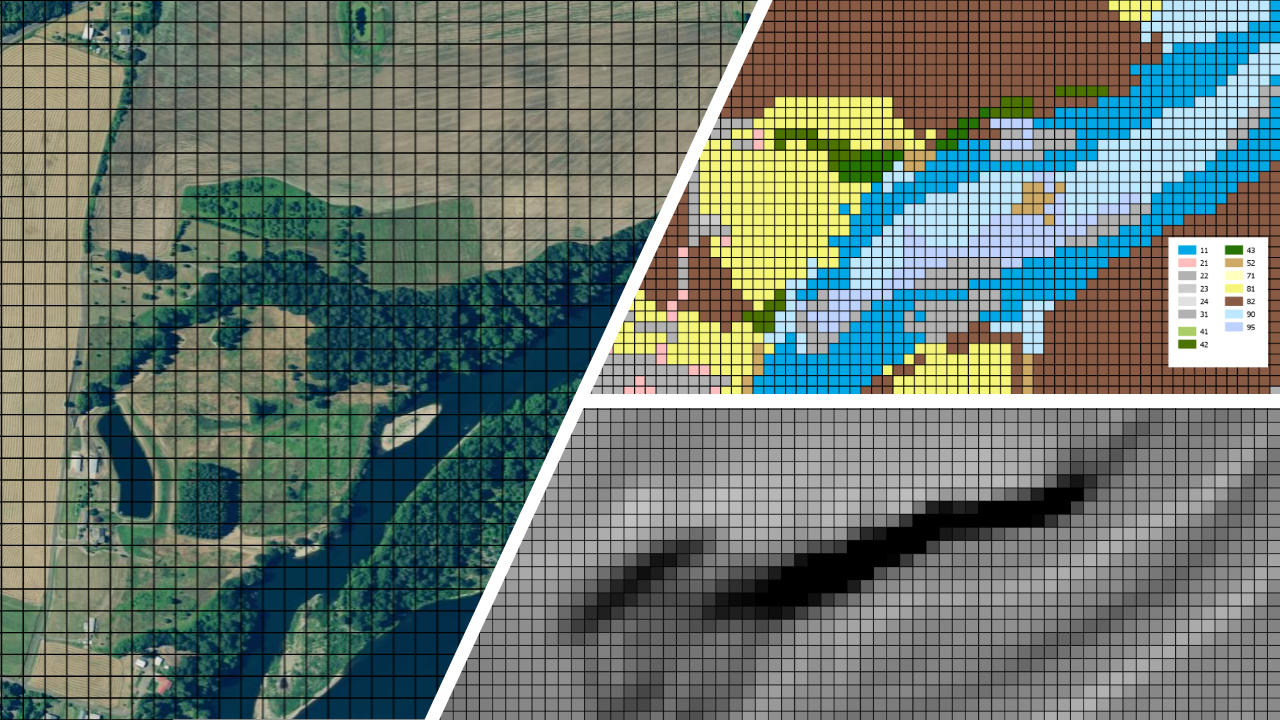
\includegraphics[width=1\linewidth]{images/Rasters4} \caption{Raster Data}\label{fig:unnamed-chunk-17}
\end{figure}

We will delve into working with each of these types of data in their own sections, but let's go over how these spatial data types are handled in R briefly.

Basic data structures in R can represent spatial data - all we need is some vectors with location and attribute information - below we generate cites with population, add a polygon, and make a map with a legend - take a minute to run this code in your own R session and make sure you understand what each line is doing.

\begin{Shaded}
\begin{Highlighting}[]
\NormalTok{cities <-}\StringTok{ }\KeywordTok{c}\NormalTok{(}\StringTok{'Ashland'}\NormalTok{,}\StringTok{'Corvallis'}\NormalTok{,}\StringTok{'Bend'}\NormalTok{,}\StringTok{'Portland'}\NormalTok{,}\StringTok{'Newport'}\NormalTok{)}
\NormalTok{longitude <-}\StringTok{ }\KeywordTok{c}\NormalTok{(}\OperatorTok{-}\FloatTok{122.699}\NormalTok{, }\FloatTok{-123.275}\NormalTok{, }\FloatTok{-121.313}\NormalTok{, }\FloatTok{-122.670}\NormalTok{, }\FloatTok{-124.054}\NormalTok{)}
\NormalTok{latitude <-}\StringTok{ }\KeywordTok{c}\NormalTok{(}\FloatTok{42.189}\NormalTok{, }\FloatTok{44.57}\NormalTok{, }\FloatTok{44.061}\NormalTok{, }\FloatTok{45.523}\NormalTok{, }\FloatTok{44.652}\NormalTok{)}
\NormalTok{population <-}\StringTok{ }\KeywordTok{c}\NormalTok{(}\DecValTok{20062}\NormalTok{,}\DecValTok{50297}\NormalTok{,}\DecValTok{61362}\NormalTok{,}\DecValTok{537557}\NormalTok{,}\DecValTok{9603}\NormalTok{)}
\NormalTok{locs <-}\StringTok{ }\KeywordTok{cbind}\NormalTok{(longitude, latitude) }
\KeywordTok{plot}\NormalTok{(locs, }\DataTypeTok{cex=}\KeywordTok{sqrt}\NormalTok{(population}\OperatorTok{*}\NormalTok{.}\DecValTok{0002}\NormalTok{), }\DataTypeTok{pch=}\DecValTok{20}\NormalTok{, }\DataTypeTok{col=}\StringTok{'red'}\NormalTok{, }
  \DataTypeTok{main=}\StringTok{'Population'}\NormalTok{, }\DataTypeTok{xlim =} \KeywordTok{c}\NormalTok{(}\OperatorTok{-}\DecValTok{124}\NormalTok{,}\OperatorTok{-}\FloatTok{120.5}\NormalTok{), }\DataTypeTok{ylim =} \KeywordTok{c}\NormalTok{(}\DecValTok{42}\NormalTok{, }\DecValTok{46}\NormalTok{))}
\KeywordTok{text}\NormalTok{(locs, cities, }\DataTypeTok{pos=}\DecValTok{4}\NormalTok{)}

\CommentTok{# Add a legend}
\NormalTok{breaks <-}\StringTok{ }\KeywordTok{c}\NormalTok{(}\DecValTok{20000}\NormalTok{, }\DecValTok{50000}\NormalTok{, }\DecValTok{60000}\NormalTok{, }\DecValTok{100000}\NormalTok{)}
\KeywordTok{options}\NormalTok{(}\DataTypeTok{scipen=}\DecValTok{3}\NormalTok{)}
\KeywordTok{legend}\NormalTok{(}\StringTok{"topright"}\NormalTok{, }\DataTypeTok{legend=}\NormalTok{breaks, }\DataTypeTok{pch=}\DecValTok{20}\NormalTok{, }\DataTypeTok{pt.cex=}\DecValTok{1}\OperatorTok{+}\NormalTok{breaks}\OperatorTok{/}\DecValTok{20000}\NormalTok{, }
  \DataTypeTok{col=}\StringTok{'red'}\NormalTok{, }\DataTypeTok{bg=}\StringTok{'gray'}\NormalTok{)}

\CommentTok{# Add polygon}
\NormalTok{lon <-}\StringTok{ }\KeywordTok{c}\NormalTok{(}\OperatorTok{-}\FloatTok{123.5}\NormalTok{, }\FloatTok{-123.5}\NormalTok{, }\FloatTok{-122.5}\NormalTok{, }\FloatTok{-122.670}\NormalTok{, }\DecValTok{-123}\NormalTok{)}
\NormalTok{lat <-}\StringTok{ }\KeywordTok{c}\NormalTok{(}\DecValTok{43}\NormalTok{, }\FloatTok{45.5}\NormalTok{, }\DecValTok{44}\NormalTok{, }\DecValTok{43}\NormalTok{, }\DecValTok{43}\NormalTok{)}
\NormalTok{x <-}\StringTok{ }\KeywordTok{cbind}\NormalTok{(lon, lat)}
\KeywordTok{polygon}\NormalTok{(x, }\DataTypeTok{border=}\StringTok{'blue'}\NormalTok{)}
\KeywordTok{lines}\NormalTok{(x, }\DataTypeTok{lwd=}\DecValTok{3}\NormalTok{, }\DataTypeTok{col=}\StringTok{'red'}\NormalTok{)}
\KeywordTok{points}\NormalTok{(x, }\DataTypeTok{cex=}\DecValTok{2}\NormalTok{, }\DataTypeTok{pch=}\DecValTok{20}\NormalTok{)}
\end{Highlighting}
\end{Shaded}

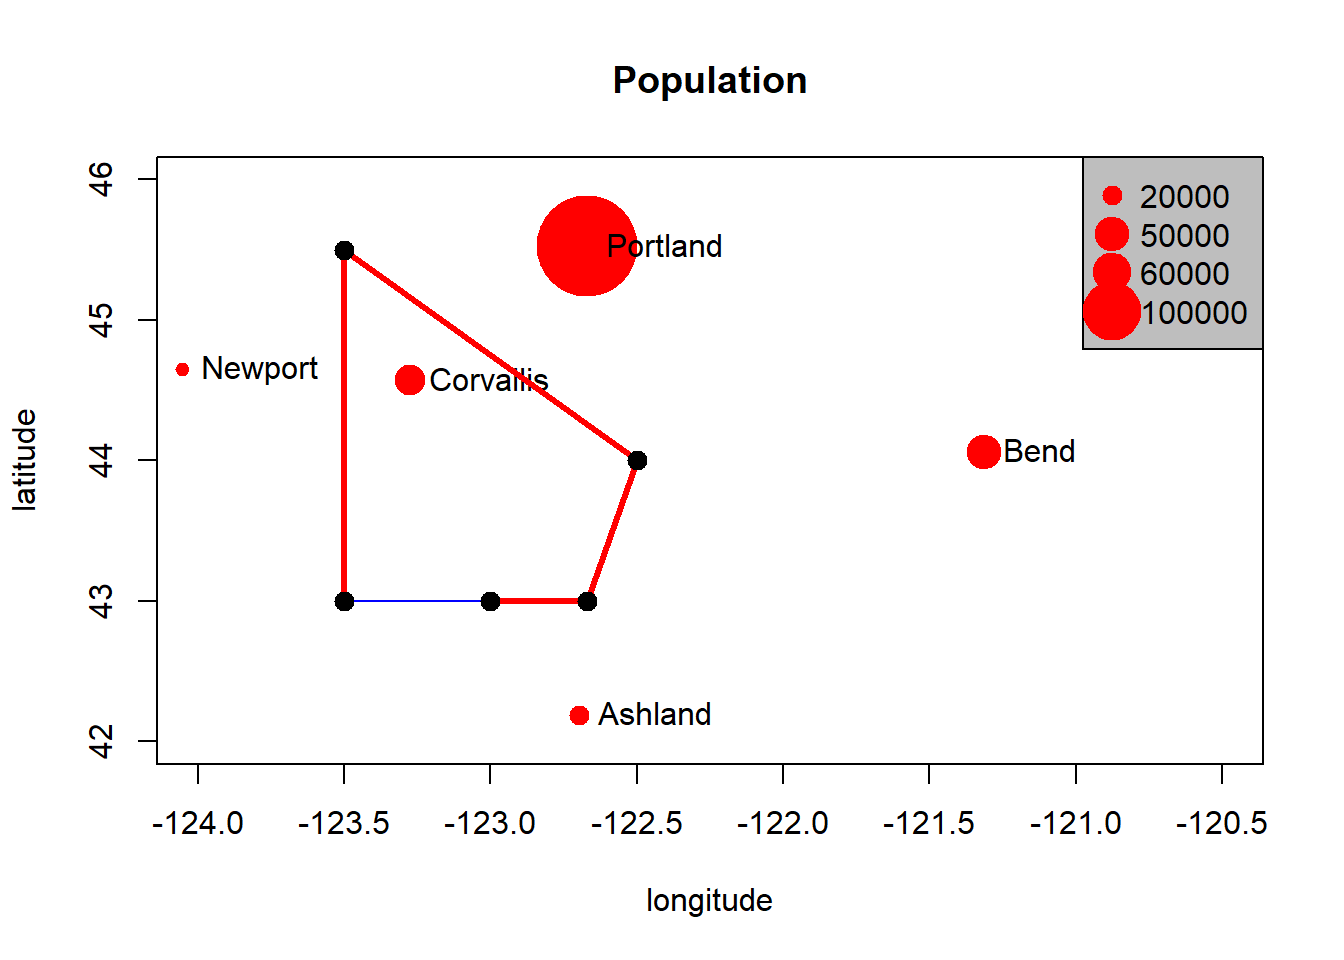
\includegraphics{AWRA_2020_R_Spatial_files/figure-latex/basic spatial data structures vector-1.pdf}

We can see in this toy example that numeric vectors can represent locations in R for simple mapping. Points just need to be a pair of numbers in cartesian space, and lines and polygons are just a number of these points (note that polygons are closed by having their first point coincide with last point which the polygon function in base R graphics takes care of).

What about raster data? A raster in essence is simply a matrix of values for raster cells

\begin{Shaded}
\begin{Highlighting}[]
\KeywordTok{library}\NormalTok{(}\StringTok{'plot.matrix'}\NormalTok{)}
\CommentTok{# numeric matrix}
\NormalTok{x <-}\StringTok{ }\KeywordTok{matrix}\NormalTok{(}\KeywordTok{runif}\NormalTok{(}\DecValTok{35}\NormalTok{), }\DataTypeTok{ncol=}\DecValTok{5}\NormalTok{) }\CommentTok{# create a numeric matrix object}
\KeywordTok{class}\NormalTok{(x)}
\end{Highlighting}
\end{Shaded}

\begin{verbatim}
## [1] "matrix" "array"
\end{verbatim}

\begin{Shaded}
\begin{Highlighting}[]
\CommentTok{#> [1] "matrix"}
\KeywordTok{par}\NormalTok{(}\DataTypeTok{mar=}\KeywordTok{c}\NormalTok{(}\FloatTok{5.1}\NormalTok{, }\FloatTok{4.1}\NormalTok{, }\FloatTok{4.1}\NormalTok{, }\FloatTok{4.1}\NormalTok{)) }\CommentTok{# adapt margins}
\KeywordTok{plot}\NormalTok{(x)}
\end{Highlighting}
\end{Shaded}

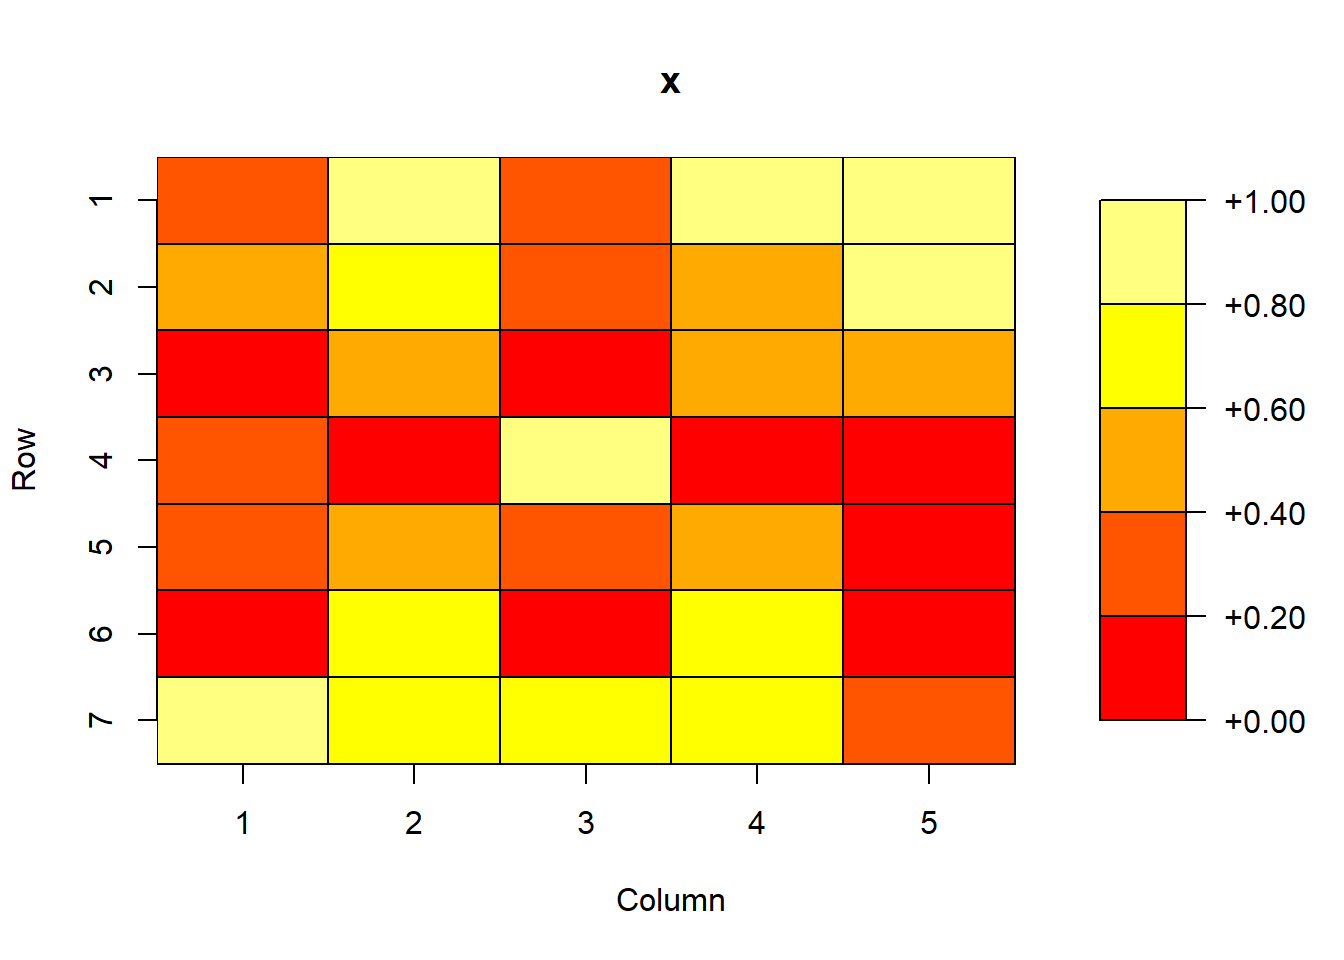
\includegraphics{AWRA_2020_R_Spatial_files/figure-latex/basic spatial data structures raster-1.pdf}

We have a `raster' of cell values in columnns and rows - but what is lacking?

You can do simple things with these spatial representations using basic R structures, but it breaks down quickly if you want to ask any spatial questions - for instance using the first example above, how would we figure out the nearest city to Corvallis? Or imagine the polygon is a county and we wanted to know what cities are within the county? Or how would we superimpose our cities on our raster cells? Or extract the value of a cell at the location of a city?

\hypertarget{challenge}{%
\subsection{Challenge}\label{challenge}}

What information do we need to properly define spatial vector data and perform spatial operations?

\hypertarget{answer}{%
\subsection{Answer}\label{answer}}

\begin{itemize}
\tightlist
\item
  A coordinate reference system (CRS)
\item
  A bounding box or extent
\item
  Methods for storing and accessing spatial attributes of data
\item
  ?
\end{itemize}

\hypertarget{r-spatial-package-landscape}{%
\subsection{R Spatial Package Landscape}\label{r-spatial-package-landscape}}

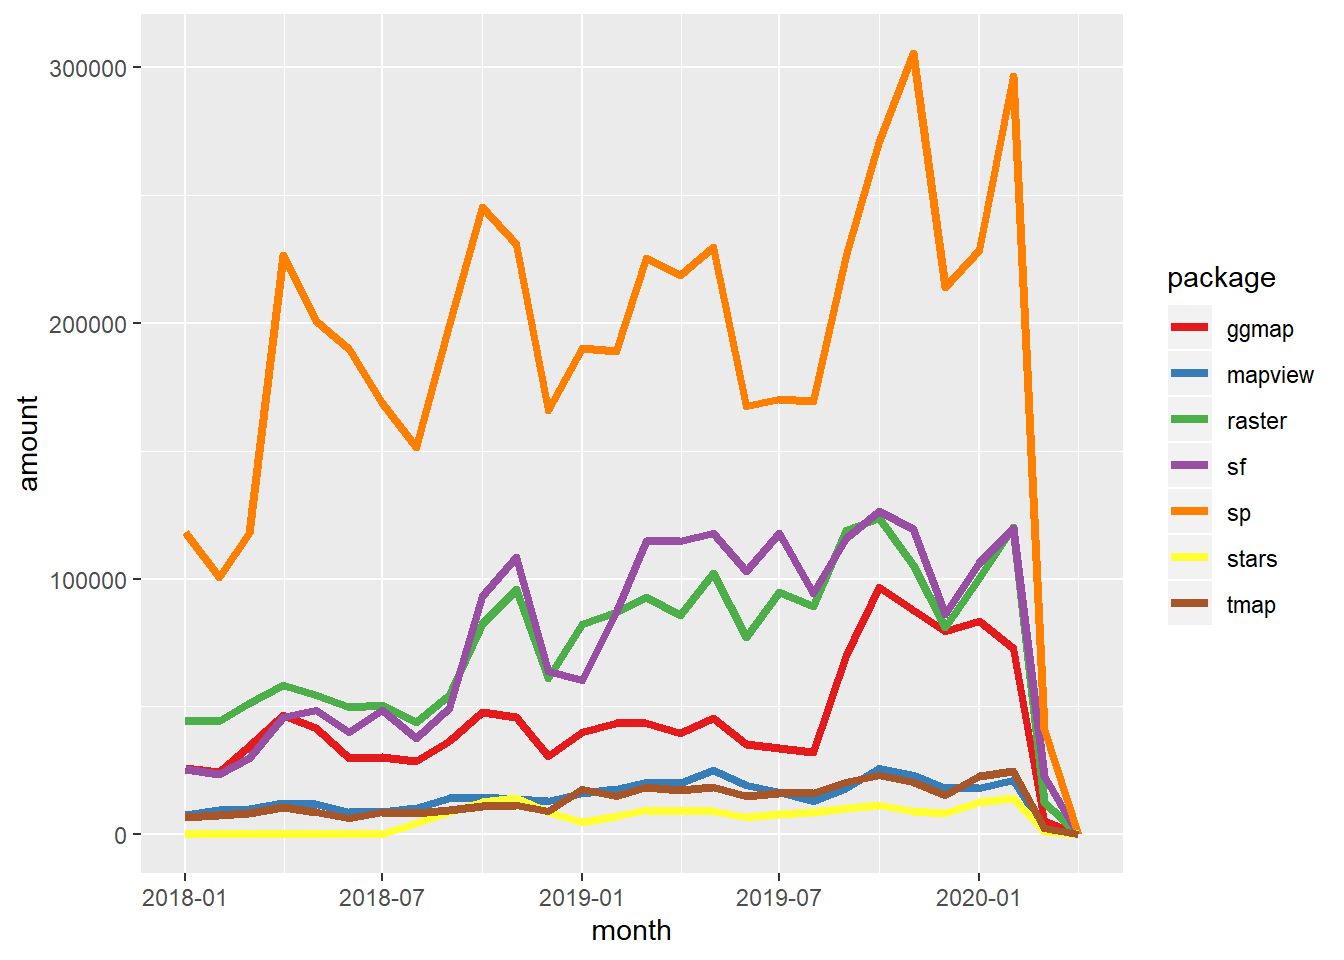
\includegraphics{AWRA_2020_R_Spatial_files/figure-latex/spatial packages-1.pdf}

\hypertarget{how-did-we-make-this-figure}{%
\subsection{How did we make this figure?}\label{how-did-we-make-this-figure}}

Look at answer below, run code in your own code editor, see if it makes sense and ask questions

\hypertarget{answer-1}{%
\subsection{Answer}\label{answer-1}}

\begin{Shaded}
\begin{Highlighting}[]
\CommentTok{# devtools::install_github("metacran/cranlogs")}
\KeywordTok{library}\NormalTok{(cranlogs, }\DataTypeTok{quietly =}\NormalTok{ T)}
\KeywordTok{library}\NormalTok{(ggplot2, }\DataTypeTok{quietly =}\NormalTok{ T)}
\KeywordTok{library}\NormalTok{(lubridate, }\DataTypeTok{quietly =}\NormalTok{ T)}
\KeywordTok{library}\NormalTok{(dplyr, }\DataTypeTok{quietly =}\NormalTok{ T)}
\KeywordTok{options}\NormalTok{(}\DataTypeTok{scipen=}\DecValTok{3}\NormalTok{)}
\NormalTok{stats <-}\StringTok{ }\KeywordTok{cran_downloads}\NormalTok{(}\DataTypeTok{from =} \StringTok{"2018-01-01"}\NormalTok{, }\DataTypeTok{to =} \StringTok{"2020-04-01"}\NormalTok{,}\DataTypeTok{packages =} \KeywordTok{c}\NormalTok{(}\StringTok{"sp"}\NormalTok{, }\StringTok{"sf"}\NormalTok{, }\StringTok{"raster"}\NormalTok{, }\StringTok{"tmap"}\NormalTok{, }\StringTok{"mapview"}\NormalTok{, }\StringTok{"leaflet"}\NormalTok{, }\StringTok{"ggmap"}\NormalTok{, }\StringTok{"stars"}\NormalTok{))}

\NormalTok{monthly_stats <-}\StringTok{ }\NormalTok{stats }\OperatorTok\StringTok{ }
\StringTok{  }\KeywordTok{group_by}\NormalTok{(}\DataTypeTok{month=}\KeywordTok{floor_date}\NormalTok{(date, }\StringTok{"month"}\NormalTok{), package) }\OperatorTok
\StringTok{  }\KeywordTok{summarize}\NormalTok{(}\DataTypeTok{amount=}\KeywordTok{sum}\NormalTok{(count))}
\KeywordTok{ggplot}\NormalTok{(monthly_stats, }\KeywordTok{aes}\NormalTok{(}\DataTypeTok{x=}\NormalTok{month, }\DataTypeTok{y=}\NormalTok{amount, }\DataTypeTok{group =}\NormalTok{ package, }\DataTypeTok{colour =}\NormalTok{ package)) }\OperatorTok{+}\StringTok{ }\KeywordTok{geom_line}\NormalTok{(}\DataTypeTok{size=}\FloatTok{1.5}\NormalTok{) }\OperatorTok{+}\StringTok{ }\KeywordTok{scale_colour_brewer}\NormalTok{(}\DataTypeTok{palette=}\StringTok{"Set1"}\NormalTok{) }\OperatorTok{+}\StringTok{ }\KeywordTok{ggtitle}\NormalTok{(}\StringTok{"R Monthly Spatial Package }\CharTok{\textbackslash{}n}\StringTok{ Downloads since 2018"}\NormalTok{)}
\end{Highlighting}
\end{Shaded}

\hypertarget{primary-r-spatial-packages}{%
\subsection{Primary R spatial packages}\label{primary-r-spatial-packages}}

\begin{figure}
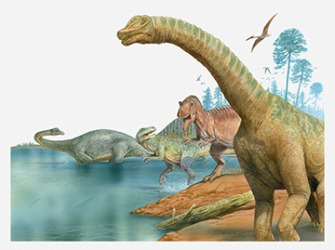
\includegraphics[width=0.75\linewidth]{images/Prehistoric} \caption{Moving on from `sp`}\label{fig:unnamed-chunk-18}
\end{figure}

\texttt{sp} was the core vector spatial data package in R for a number of years, and while still used and while many packages still depend on the package, we will make a clean break in this workshop and focus entirely on the new \texttt{sf} package for working with vector data.

This portion of the workshop will focus primarily on the following core packages for working with spatial data in R:
- \texttt{sf} - The core package for working with vector data in R
- \texttt{raster} - Still the primary spatial package for working with raster data in R
- \texttt{mapview} - this is a wrapper package for R \texttt{leaflet} package and I find simpler and more intuitive
- \texttt{ggolot} and \texttt{tmap} - static plotting and thematic maping
- \texttt{dplyr} - Not a spatial package, but \texttt{sf} is ``tidy-compliant'' and we will follow ``tidy'' workflows in this portion of the workshop for much or our examples

The \href{https://cran.r-project.org/web/views/Spatial.html}{R Spatial Task View page} provides current and comprehensive information on the ecosystem of R packages for working with spatial data - there are hundreds out there for specific tasks - we'll touch on several others besides core packages above this morning.

\hypertarget{quick-examples}{%
\section{Quick examples}\label{quick-examples}}

Here is just a sampling of few quick spatial tasks.

\hypertarget{geocoding-example-with-tmaptools-using-open-street-map}{%
\subsection{Geocoding example with tmaptools using open street map}\label{geocoding-example-with-tmaptools-using-open-street-map}}

Here we'll use the \texttt{tmap} package and \texttt{tmaptools} to `geocode' a named feature in OpenStreetMap import it into our R session as an \texttt{sf} feature.

\begin{Shaded}
\begin{Highlighting}[]
\CommentTok{# uses OSM}
\KeywordTok{library}\NormalTok{(tmap)}
\KeywordTok{library}\NormalTok{(tmaptools)}
\KeywordTok{library}\NormalTok{(dplyr)}
\NormalTok{tex_cap <-tmaptools}\OperatorTok{::}\KeywordTok{geocode_OSM}\NormalTok{(}\StringTok{"Texas Capital"}\NormalTok{, }
        \DataTypeTok{as.sf =} \OtherTok{TRUE}\NormalTok{) }\OperatorTok\StringTok{ }
\StringTok{  }\KeywordTok{glimpse}\NormalTok{()}
\end{Highlighting}
\end{Shaded}

\begin{verbatim}
## Rows: 1
## Columns: 9
## $ query   <chr> "Texas Capital"
## $ lat     <dbl> -31.46748
## $ lon     <dbl> -64.22844
## $ lat_min <dbl> -31.46748
## $ lat_max <dbl> -31.46748
## $ lon_min <dbl> -64.22995
## $ lon_max <dbl> -64.22723
## $ bbox    <POLYGON [°]> POLYGON ((-64.22995 -31.467...
## $ point   <POINT [°]> POINT (-64.22844 -31.46748)
\end{verbatim}

\hypertarget{run-and-examine-code-chunk-above}{%
\subsection{Run and examine code chunk above}\label{run-and-examine-code-chunk-above}}

\begin{enumerate}
\def\labelenumi{\arabic{enumi}.}
\tightlist
\item
  What is the double colon doing?
\item
  What is the \texttt{geocode\_OSM} function doing?
\item
  Explain how the code runs together using the \texttt{\%\textgreater{}\%} chaining operator
\item
  What is \texttt{glimpse}? Is it useful compared to \texttt{head} function?
\end{enumerate}

\hypertarget{answer-2}{%
\subsection{Answer}\label{answer-2}}

\begin{enumerate}
\def\labelenumi{\arabic{enumi}.}
\tightlist
\item
  It specifies using \texttt{geocode\_OSM} from the \texttt{tmaptools} package. R gives namespace preference to packages in order loaded; some packages share function names; so it's good practice to disambiguate your functions with the double-colon
\item
  It is looking up a named feature in OpenStreetMap and returning the coordinates (bonus - we'll delve into more in next section - what coordinate reference system are coordinates in and how to you find out?)
\item
  You would translate code using the \texttt{\textgreater{}\%\textgreater{}} operator from:
\end{enumerate}

\begin{itemize}
\tightlist
\item
  do this \texttt{\%\textgreater{}\%} do that \texttt{\%\textgreater{}\%} do that
\end{itemize}

To

\begin{itemize}
\tightlist
\item
  do this \emph{then} do that \emph{then} do that
\end{itemize}

\begin{enumerate}
\def\labelenumi{\arabic{enumi}.}
\setcounter{enumi}{3}
\tightlist
\item
  Technically, it's a transposed version of \texttt{print} - columns run down page, data across like rows - it additionally gives you the number of observations and variables, and the data type of each column
\end{enumerate}

\begin{itemize}
\tightlist
\item
  bonus: how would you quickly learn more about \texttt{glimpse} from the console?
\end{itemize}

\hypertarget{interactive-mapping}{%
\subsection{Interactive mapping}\label{interactive-mapping}}

\begin{Shaded}
\begin{Highlighting}[]
\KeywordTok{library}\NormalTok{(mapview)}
\KeywordTok{mapview}\NormalTok{(tex_cap)}
\end{Highlighting}
\end{Shaded}

\begin{verbatim}
## PhantomJS not found. You can install it with webshot::install_phantomjs(). If it is installed, please make sure the phantomjs executable can be found via the PATH variable.
\end{verbatim}

\hypertarget{htmlwidget-86bd956c9d925816aaf7}{}
\begin{leaflet}

\end{leaflet}

\hypertarget{choropleth-map}{%
\subsection{Choropleth map}\label{choropleth-map}}

The excellent \texttt{tigris} package can be used to get census boundaries such as states and counties as vector \texttt{sf} objects in R

\begin{Shaded}
\begin{Highlighting}[]
\KeywordTok{library}\NormalTok{(sf)}
\KeywordTok{library}\NormalTok{(tigris)}
\NormalTok{counties <-}\StringTok{ }\KeywordTok{counties}\NormalTok{(}\StringTok{"Texas"}\NormalTok{, }\DataTypeTok{cb =} \OtherTok{TRUE}\NormalTok{)}
\NormalTok{counties}\OperatorTok{$}\NormalTok{area <-}\StringTok{ }\KeywordTok{as.numeric}\NormalTok{(}\KeywordTok{st_area}\NormalTok{(counties))}
\KeywordTok{glimpse}\NormalTok{(counties)}

\KeywordTok{tm_shape}\NormalTok{(counties) }\OperatorTok{+}
\StringTok{  }\KeywordTok{tm_polygons}\NormalTok{(}\StringTok{"area"}\NormalTok{, }
              \DataTypeTok{style=}\StringTok{"quantile"}\NormalTok{, }
              \DataTypeTok{title=}\StringTok{"Texas Counties Area"}\NormalTok{)}
\end{Highlighting}
\end{Shaded}

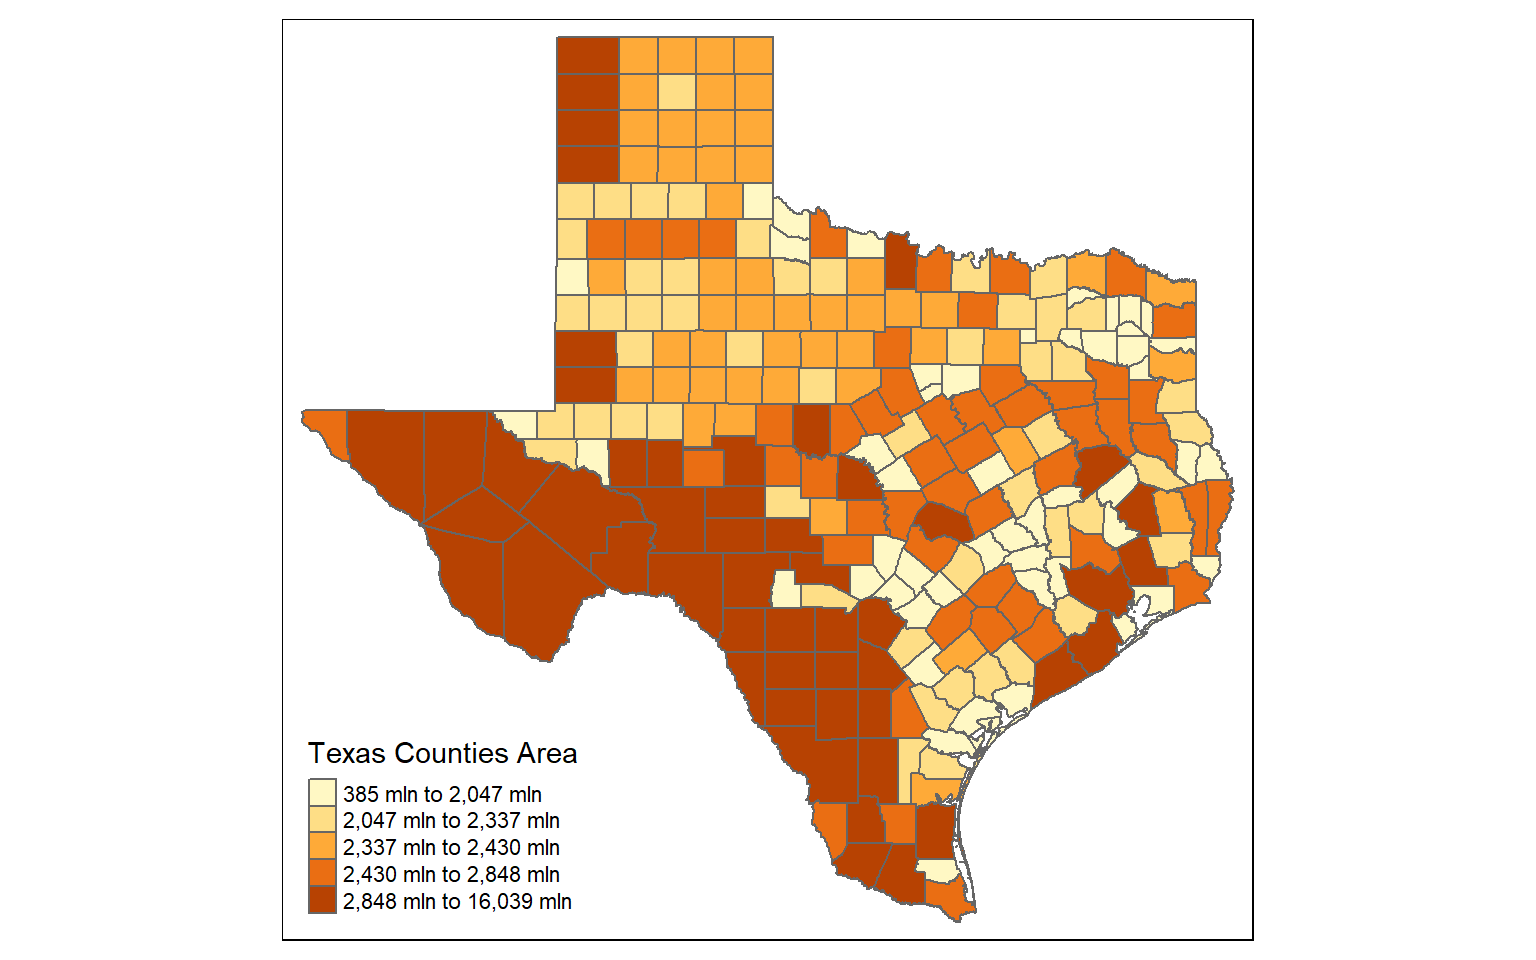
\includegraphics{AWRA_2020_R_Spatial_files/figure-latex/tmap example-1.pdf}

\hypertarget{a-little-about-coordinate-reference-systems}{%
\chapter{A little about coordinate reference systems}\label{a-little-about-coordinate-reference-systems}}

\hypertarget{vector-data-with-sf}{%
\chapter{Vector data with sf}\label{vector-data-with-sf}}

\begin{itemize}
\tightlist
\item
  Some key aspects of sf
\end{itemize}

\begin{figure}
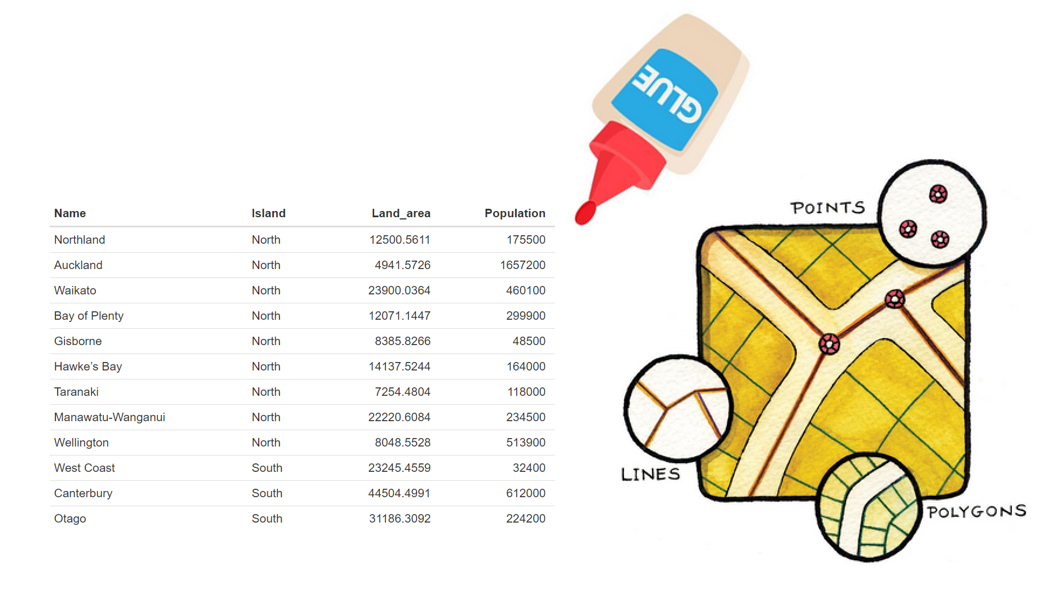
\includegraphics[width=1.5\linewidth]{images/Sticky} \caption{Sticky geometry with `sf`}\label{fig:unnamed-chunk-19}
\end{figure}

Load \texttt{tidycensus} - you'll need to set your Census API key. A key can be obtained from \href{http://api.census.gov/data/key_signup.html}{here}.

\begin{Shaded}
\begin{Highlighting}[]
\KeywordTok{library}\NormalTok{(sf)}
\KeywordTok{library}\NormalTok{(tidycensus)}
\KeywordTok{library}\NormalTok{(tidyverse)}
\CommentTok{# census_api_key("YOUR API KEY GOES HERE")}
\end{Highlighting}
\end{Shaded}

\begin{Shaded}
\begin{Highlighting}[]
\KeywordTok{library}\NormalTok{(tidycensus)}
\KeywordTok{library}\NormalTok{(ggplot2)}
\KeywordTok{options}\NormalTok{(}\DataTypeTok{tigris_use_cache =} \OtherTok{TRUE}\NormalTok{)}
\NormalTok{austin_tracts <-}\StringTok{ }\KeywordTok{get_acs}\NormalTok{(}\DataTypeTok{state =} \StringTok{'TX'}\NormalTok{, }\DataTypeTok{county =} \StringTok{'Travis'}\NormalTok{, }\DataTypeTok{geography =} \StringTok{"tract"}\NormalTok{,}
                         \DataTypeTok{variables =} \StringTok{"B19013_001"}\NormalTok{, }\DataTypeTok{geometry =} \OtherTok{TRUE}\NormalTok{)}
\end{Highlighting}
\end{Shaded}

\begin{verbatim}
## Getting data from the 2014-2018 5-year ACS
\end{verbatim}

\begin{Shaded}
\begin{Highlighting}[]
\NormalTok{austin_tracts }\OperatorTok
\StringTok{  }\KeywordTok{ggplot}\NormalTok{(}\KeywordTok{aes}\NormalTok{(}\DataTypeTok{fill =}\NormalTok{ estimate)) }\OperatorTok{+}\StringTok{ }
\StringTok{  }\KeywordTok{geom_sf}\NormalTok{(}\DataTypeTok{color =} \OtherTok{NA}\NormalTok{) }\OperatorTok{+}\StringTok{ }
\StringTok{  }\KeywordTok{coord_sf}\NormalTok{(}\DataTypeTok{crs =} \DecValTok{26911}\NormalTok{) }\OperatorTok{+}\StringTok{ }
\StringTok{  }\KeywordTok{scale_fill_viridis_c}\NormalTok{(}\DataTypeTok{option =} \StringTok{"magma"}\NormalTok{) }
\end{Highlighting}
\end{Shaded}

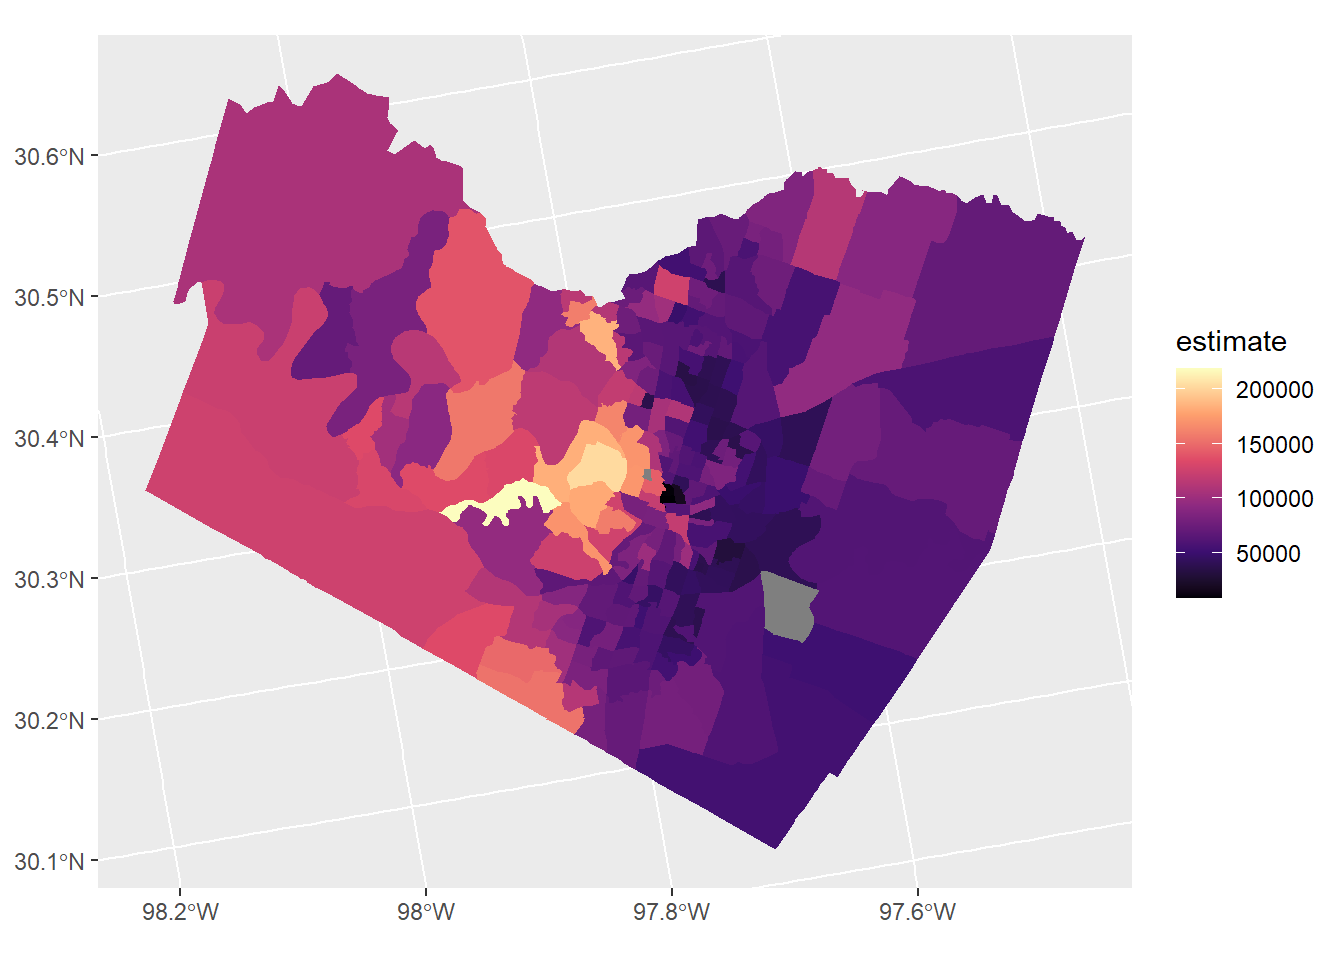
\includegraphics{AWRA_2020_R_Spatial_files/figure-latex/unnamed-chunk-21-1.pdf}

\hypertarget{challenge-chained-spatial-operation}{%
\subsection{Challenge: Chained spatial operation}\label{challenge-chained-spatial-operation}}

Earlier we showed example of printing and storing a statement using parens

\begin{Shaded}
\begin{Highlighting}[]
\NormalTok{(file <-}\StringTok{ }\KeywordTok{system.file}\NormalTok{(}\StringTok{"gpkg/nc.gpkg"}\NormalTok{, }\DataTypeTok{package=}\StringTok{'sf'}\NormalTok{))}
\end{Highlighting}
\end{Shaded}

\begin{verbatim}
## [1] "C:/Users/mweber/R/library/sf/gpkg/nc.gpkg"
\end{verbatim}

How would we read this file into an \texttt{sf} data frame using chained operation?

\hypertarget{answer}{%
\subsection{Answer}\label{answer}}

\begin{Shaded}
\begin{Highlighting}[]
\NormalTok{(file }\OperatorTok\StringTok{ }\KeywordTok{read_sf}\NormalTok{() ->}\StringTok{ }\NormalTok{nc)}
\end{Highlighting}
\end{Shaded}

\begin{verbatim}
## Simple feature collection with 100 features and 14 fields
## geometry type:  MULTIPOLYGON
## dimension:      XY
## bbox:           xmin: -84.32385 ymin: 33.88199 xmax: -75.45698 ymax: 36.58965
## geographic CRS: NAD27
## # A tibble: 100 x 15
##     AREA PERIMETER CNTY_ CNTY_ID NAME  FIPS  FIPSNO CRESS_ID BIR74 SID74 NWBIR74
##    <dbl>     <dbl> <dbl>   <dbl> <chr> <chr>  <dbl>    <int> <dbl> <dbl>   <dbl>
##  1 0.114      1.44  1825    1825 Ashe  37009  37009        5  1091     1      10
##  2 0.061      1.23  1827    1827 Alle~ 37005  37005        3   487     0      10
##  3 0.143      1.63  1828    1828 Surry 37171  37171       86  3188     5     208
##  4 0.07       2.97  1831    1831 Curr~ 37053  37053       27   508     1     123
##  5 0.153      2.21  1832    1832 Nort~ 37131  37131       66  1421     9    1066
##  6 0.097      1.67  1833    1833 Hert~ 37091  37091       46  1452     7     954
##  7 0.062      1.55  1834    1834 Camd~ 37029  37029       15   286     0     115
##  8 0.091      1.28  1835    1835 Gates 37073  37073       37   420     0     254
##  9 0.118      1.42  1836    1836 Warr~ 37185  37185       93   968     4     748
## 10 0.124      1.43  1837    1837 Stok~ 37169  37169       85  1612     1     160
## # ... with 90 more rows, and 4 more variables: BIR79 <dbl>, SID79 <dbl>,
## #   NWBIR79 <dbl>, geom <MULTIPOLYGON [°]>
\end{verbatim}

A question to use on a spatial tibble - What type of object is '`? If you \texttt{run\ head()} does it behave the way you're used to seeing \texttt{head} function? How might you get the behavior you're used to seeing from \texttt{head} with''

\hypertarget{raster-data}{%
\chapter{Raster data}\label{raster-data}}

\hypertarget{geoprocessing}{%
\chapter{Geoprocessing}\label{geoprocessing}}

\hypertarget{example-one}{%
\section{Example one}\label{example-one}}

\hypertarget{example-two}{%
\section{Example two}\label{example-two}}

\hypertarget{references}{%
\chapter*{References}\label{references}}
\addcontentsline{toc}{chapter}{References}

\hypertarget{r-spatial-resources}{%
\subsection{R Spatial Resources}\label{r-spatial-resources}}

\begin{itemize}
\tightlist
\item
  \href{http://rspatial.org/spatial/}{R Spatial - \textbf{Spatial Data Science with R}}
\item
  \href{https://geocompr.robinlovelace.net/}{\textbf{Geocomputation with R}}
\item
  \href{https://cran.r-project.org/web/views/Spatial.html}{\textbf{R Spatial Task View}}
\item
  \href{http://files.zevross.com/workshops/spatial/slides/html/0-deck-list.html}{\textbf{Modern Geospatial Data Analysis with R by Zev Ross}}
\item
  \href{https://keen-swartz-3146c4.netlify.com/}{\textbf{Spatial Data Science - Pebesma and Bivand}}
\item
  \href{http://adamwilson.us/SpatialDataScience/index.html}{\textbf{Spatial Data Science Course- Prof.~Adam Wilson}}
\item
  \href{https://cengel.github.io/rspatial/}{\textbf{Introduction to Mapping and Spatial Analysis with R}}
\item
  \href{https://mhweber.github.io/R-User-Group-Spatial-Workshop-2018/index.html}{\textbf{R Spatial Workshop for EPA R User Group}}
\item
  \href{https://mgimond.github.io/Spatial/index.html}{\textbf{Intro to GIS and Spatial Analysis by Manuel Gimond}}
\item
  \href{https://bakaniko.github.io/FOSS4G2019_Geoprocessing_with_R_workshop/}{\textbf{FOSS4G2019 R for Geospatial Processing}}
\item
  \href{https://bookdown.org/lexcomber/brunsdoncomber2e/}{\textbf{An Introduction to Spatial Analysis and Mapping in R}}
\end{itemize}

\hypertarget{r-vector-processing-simple-features-resources}{%
\subsection{R Vector Processing / Simple Features Resources}\label{r-vector-processing-simple-features-resources}}

\begin{itemize}
\tightlist
\item
  \href{https://r-spatial.github.io/sf/index.html}{\textbf{Simple Features for R}}
\item
  \href{https://edzer.github.io/UseR2017/}{\textbf{Spatial Data in R: New Directions}}
\item
  \href{https://github.com/r-spatial/sf/wiki/Migrating}{\textbf{sp-sf Migration}}
\item
  \href{https://www.jessesadler.com/post/simple-feature-objects/}{\textbf{An Exploration of Simple Features for R}}
\item
  \href{https://www.azavea.com/blog/2017/08/30/spatial-analysis-pipelines-in-r-with-simple-features/}{\textbf{Simple Features: Building Spatial Data Pipelines in R}}
\item
  \href{http://strimas.com/r/tidy-sf/}{\textbf{Tidy spatial data in R: using dplyr, tidyr, and ggplot2 with sf}}
\end{itemize}

\hypertarget{r-raster-resources}{%
\subsection{R Raster Resources}\label{r-raster-resources}}

\begin{itemize}
\tightlist
\item
  \href{http://geoscripting-wur.github.io/IntroToRaster/}{Wageningen University \textbf{Intro to Raster}}
\item
  \href{https://geoscripting-wur.github.io/AdvancedRasterAnalysis/}{Wageningen University \textbf{Advanced Raster Analysis}}
\item
  \href{https://github.com/etiennebr/visualraster}{\textbf{The Visual Raster Cheat Sheet GitHub Repo}}
\item
  \href{https://oscarperpinan.github.io/rastervis/}{\textbf{Rastervis}}
\item
  \href{https://r-spatial.github.io/stars/}{\textbf{stars - spatiotemporal arrays}}
\end{itemize}

\hypertarget{r-mapping-resources}{%
\subsection{R Mapping Resources}\label{r-mapping-resources}}

\begin{itemize}
\tightlist
\item
  \href{https://r-spatial.github.io/mapview/}{\textbf{mapview}}
\item
  \href{https://rstudio.github.io/leaflet/}{\textbf{Leaflet for R}}
\item
  \href{https://github.com/mtennekes/tmap}{\textbf{tmap}}
\item
  \href{http://zevross.com/blog/2018/10/02/creating-beautiful-demographic-maps-in-r-with-the-tidycensus-and-tmap-packages/}{Zev Ross \textbf{Creating beautiful demographic maps in R with the \texttt{tidycensus} and \texttt{tmap} packages}}
\item
  \href{https://geocompr.robinlovelace.net/adv-map.html}{Geocomputation with R: \textbf{Making maps with R}}
\item
  \href{https://ryanpeek.github.io/mapping-in-R-workshop/index.html}{Ryan Peek: \textbf{Mapping in R}}
\end{itemize}

\hypertarget{general-r-resources}{%
\subsection{General R Resources}\label{general-r-resources}}

\begin{itemize}
\tightlist
\item
  \href{https://google.github.io/styleguide/Rguide.xml}{\textbf{Google R Style Guide}}
\item
  \href{http://adv-r.had.co.nz/}{\textbf{Advanced R by Hadley Wickham}}
\end{itemize}

\end{document}
